%%	SECCION documentclass																									 %%	
%%---------------------------------------------------------------------------%%
\documentclass{report}

%%---------------------------------------------------------------------------%%
%%	SECCION usepackage																											 %%	
%%---------------------------------------------------------------------------%%
\usepackage{amsmath, amsthm}
\usepackage[spanish,activeacute]{babel}
\usepackage{caratula}
\usepackage{a4wide}
\usepackage{hyperref}
\usepackage{fancyhdr}
% \usepackage{moreverb}
\usepackage{graphicx} % Para el logo magico!
\usepackage{capt-of}
\usepackage{afterpage}
\usepackage{float}
\usepackage{amssymb}
\usepackage{amsmath}
\usepackage[latin1]{inputenc}
\usepackage{subfigure}
\usepackage{algorithm}
\usepackage{algorithmic}
\usepackage[dvipsnames,usenames]{color}
\usepackage{amsfonts}
\usepackage{pdflscape}
%%---------------------------------------------------------------------------%%
%%	SECCION opciones																												 %%	
%%---------------------------------------------------------------------------%%
\parskip    = 11 pt
\headheight	= 13.1pt
\pagestyle	{fancy}
\definecolor{orange}{rgb}{1,0.5,0}

\addtolength{\headwidth}{1.0in}

\addtolength{\oddsidemargin}{-0.5in}
\addtolength{\textwidth}{1.0in}
\addtolength{\topmargin}{-0.8in}
\addtolength{\textheight}{0.7in}

%%---------------------------------------------------------------------------%%
%%	SECCION document	 %%	
%%---------------------------------------------------------------------------%%
\begin{document}
\renewcommand{\chaptername}{Parte }
\renewcommand{\algorithmicrequire}{\textcolor{blue}{\textbf{Requiere:}}}
\renewcommand{\algorithmicensure}{\textbf{Asegura:}}
\renewcommand{\algorithmicend}{\textbf{Fin}}
\renewcommand{\algorithmicif}{\textcolor{blue}{\textbf{Si}}}
\renewcommand{\algorithmicthen}{\textcolor{blue}{\textbf{entonces}}}
\renewcommand{\algorithmicelse}{\textcolor{red}{\textbf{Si no}}}
\renewcommand{\algorithmicelsif }{\textcolor{blue}{\textbf{Si no y}}}
\renewcommand{\algorithmicendif}{\textcolor{blue}{\textbf{Fin si}}}
\renewcommand{\algorithmicfor}{\textcolor{ForestGreen}{\textbf{Para}}}
\renewcommand{\algorithmicendfor}{\textcolor{ForestGreen}{\textbf{Fin para}}}
\renewcommand{\algorithmicwhile}{\textcolor{ForestGreen}{\textbf{Mientras}}}
\renewcommand{\algorithmicendwhile}{\textcolor{ForestGreen}{\textbf{Fin mientras}}}
\renewcommand{\algorithmicdo}{\textcolor{ForestGreen}{\textbf{hacer}}}
\renewcommand{\algorithmicreturn}{\textbf{Devolver}}
\floatname{algorithm}{Algoritmo}

%%---- Caratula -------------------------------------------------------------%%
\materia{Redes :-) (2008)}
\titulo{Resumen Loco}

\integrante{Mart'inez, Federico}{3.14/0}{federicoemartinez@gmail.com}

\grupo{Grupo abeliano}
\resumen{
un resumen
}

% TOC, usa estilos locos
\maketitle
\pagestyle{empty}
{
\fancypagestyle{plain}
    {
    \fancyhead{}
    \fancyfoot{}
    \renewcommand{\headrulewidth}{0.0pt}
    } % clear header and footer of plain page because of ToC
\tableofcontents
}


\newpage
% arreglos los estilos para el resto del documento, y
% reseteo los numeros de pagina para que queden bien
\pagenumbering{arabic}
\fancypagestyle{plain} {
    \fancyhead[LO]{Mart�nez}
    \fancyhead[C]{}
    \fancyhead[RO]{P\'agina \thepage\ de \pageref{LastPage}}
    \fancyfoot{}
    \renewcommand{\headrulewidth}{0.4pt}
}
\pagestyle{plain}

\setcounter{section}{1}
\setcounter{chapter}{0}
\chapter{Alcance de la soluci�n} 

El sistema se encarga de monitorear el ciclo de vida de los pedidos que se realizan a la pizzer�a y el stock de las materias primas. Es responsable tambi�n de la optimizaci�n del uso del horno, la estimaci�n de lapsos de producci�n y entrega, y por �ltimo de conservar un registro de los eventos de inter�s con fines estad�sticos. 

En el caso de los pedidos realizados remotamente (v�a Web o SMS), el sistema se encarga tambi�n de su ingreso. Para los pedidos realizados de forma directa (ya sea a un mesero o llamando por tel�fono) existir� un inviduo responsable de su ingreso.

Desde el momento del ingreso de los pedidos, el sistema verifica su factibilidad en funci�n del stock de insumos y de disponibilidad de productos preparados con antelaci�n. Una vez ingresados los pedidos, el sistema actualiza la informaci�n de stock inmediatamente (y at�micamente junto con la inserci�n del pedido). A continuaci�n se inserta el pedido en la cola (seg�n una pol�tica predefinida por el encargado) y se presenta a quien ingres� el pedido (usuario o encargado) una estimaci�n de la demora en la preparaci�n del pedido.

Dentro de la cocina, los maestros pizzero y empanadero tienen acceso al sistema en el cual pueden observar los pedidos que deben preparar e indicar su estado de preparaci�n (en espera, preparado, en el horno, listo). El sistema les indica tambi�n qu� sector del horno corresponde para la cocci�n del pedido. Tras la preparaci�n, si el pedido debe ser entregado el sistema contin�a monitoreando su estado y la demora en la entrega, tras la cual se recibe una notificaci�n por parte del delivery. Cuando corresponda, el sistema podr� (mediante una interfaz con el sistema de facturaci�n) realizar el cobro del pedido y registrar su pago.

En todo momento el encargado puede reordenar la cola de pedidos, o cancelar alguno de ellos, as� como los usuarios pueden consultar el estado de los mismos (v�a Web o SMS). Tambi�n se puede actualizar el stock de insumos y consultar las estad�sticas y algunos �ndices del rendimiento del proceso de producci�n y entrega.

El sistema no es responsable de la log�stica de la distribuci�n ni de la interacci�n directa con los clientes que no utilizan los medios Web o SMS. Tampoco existen operaciones automatizadas que afecten al negocio: todo lo que el sistema hace es coordinar a los actores que participan. El proceso de preparaci�n y cocci�n de los alimentos es totalmente manual, as� como lo es la reposici�n del stock y el armado de los pedidos para su posterior entrega.
\chapter{Propuestas de mejora}

\section{Mejoras al proceso de producci�n y atenci�n}

La implementaci�n de un sistema inform�tico para la gesti�n del negocio incluye una serie de mejoras inherentes que contribuyen a mejorar el rendimiento del negocio:
\begin{itemize}
\item El control sistem�tico del stock
\item	El seguimiento individual de cada pedido
\item	La planificaci�n algor�tmica del uso del horno
\item	La posibilidad de tomar pedidos remotamente
\item	La posibilidad de consultar el estado de pedidos remotamente
\item	La posibilidad de pagar los pedidos remotamente
\end{itemize}

Adem�s de �stas, proponemos algunas opciones de �ndole tecnol�gica para mejorar la eficiencia en algunos aspectos:

\begin{itemize}
\item Los pedidos se env�an a la cocina mediante el sistema. Los cocineros reciben los pedidos en una interfaz touchscreen e indican cuando los est�n preparando as� como cuando los ingresaron al horno. Esto permite hacer un seguimiento fino de los pedidos.
\item Los meseros registran los pedidos en computadoras de mano y los pedidos se transfieren autom�ticamente al sistema mediante un sistema inal�mbrico, eliminando as� el paso intermedio (y potencial cuello de botella) del encargado de pedidos. As�, la tarea del encargado deja de ser funcionar como interfase entre el local  y la cocina, para pasar a ser inferfase entre los clientes que llaman por tel�fono y el sistema.
\end{itemize}

\section{Indicadores de rendimiento, estad�sticas y mejoras asociadas}

Con el fin de comprender m�s profundamente el comportamiento del negocio, desarrollamos para la pizzer�a un conjunto de indicadores que permitan analizar su rendimiento y predecir algunos de los par�metros que afectan su comportamiento, as� como optimizar algunas estrategias de venta y producci�n.

Los indicadores de rendimiento tienen por objetivo caracterizar el funcionamiento de la pizzer�a en un per�odo dado. Mediante el monitoreo de las modificaciones de estados en el sistema es posible realizar un seguimiento. Algunos par�metros interesantes pueden ser:
\begin{itemize}
\item Tasa de producci�n de la cocina
\item Tasa de ingreso de pedidos (global, y discriminados por origen del pedido)
\item Tiempo medio de espera por un pedido (discriminado seg�n local o delivery)
\item Tiempo medio de delivery (cuando corresponda)
\item Productos m�s populares
\item ``Combos'' m�s populares
\item  ``Perfiles'' de cliente
\end{itemize}

En particular, el conocimiento sobre la demanda permite mantener un menor stock de productos, disminuyendo as� el costo financiero y manteniendo una mayor eficiencia en la administraci�n de los recursos. A su vez, determinar los productos y combinaciones m�s populares puede conducir a promociones m�s efectivas, as� como a disminuciones de costos por un mejor conocimiento de los insumos necesarios para su producci�n. Por �ltimo, los perfiles de cliente permiten ejecutar estrategias de fidelizaci�n: al conocer en detalle y de forma individual las compras que realiza cada cliente se puede determinar cuales son los clientes m�s importantes y en funci�n de eso ofrecerles alg�n tipo de beneficio.

Existen otros elementos que son indicativos de la satisfacci�n de los clientes. Es interesante tambi�n medir la cantidad de cancelaciones que se producen y a qu� tipos de productos afectan, en un intento de minimizarlas ya que representan un problema para la din�mica del negocio.

Todos los indicadores propuestos pueden computarse a partir de un registro hist�rico de los eventos y cambios de estado que se producen en el sistema. Siempre con el esp�ritu de obtener informaci�n sobre el rendimiento, ideamos algunos complementos que permiten conocer algunos detalles importantes:

\begin{itemize}
\item \textbf{Confirmaci�n de entrega por SMS}:
Los responsables de delivery env�an un mensaje de texto con un c�digo de confirmaci�n para indicar que la entrega de un pedido fue exitosa. Esto permite conocer con m�s detalle el tiempo necesario para entregarle a un cliente dado, as� como el promedio de demora por entrega.
\item \textbf{Mecanismo de feedback por Internet}:
El pedido incluye un c�digo identificador que le permite al usuario, si as� lo deseara, indicar en la p�gina Web de la pizzer�a si hubo alg�n problema con su pedido (se demor� mucho, la estimaci�n de tiempo fue err�nea, la comida estaba fr�a). Esto permite no solo detectar problemas con el servicio de distribuci�n (al que es importante controlar, ya que se trata de un proveedor externo) sino tambi�n ofrecer compensaciones a los clientes damnificados.
\item \textbf{Preparaci�n adelantada de productos}:
Al disponer de estad�sticas precisas sobre la demanda que recibe el local, es posible, en funci�n de las predicciones hechas por el sistema, preparar con antelaci�n (durante momentos ociosos) los productos que se sabe que se vender�n (por ejemplo, pizzas o empanadas). Esto permite disminuir la carga de la cocina durante picos de demanda, disminuyendo as� el tama�o del staff de la pizzer�a y a su vez los costos fijos.
\end{itemize}

\chapter{Diagrama de contexto}
Dado que uno de los requerimientos hechos al sistema es que en caso de contingencia, se pueda operar desde el puesto del 
encargado de pedidos, decidimos, por consejo docente, separar el diagrama de contexto en un contexto normal y el contexto de
contingencia. %FIXME: consejo docente?

El siguiente es el diagrama de contexto de la situacion normal,  a continuaci�n una version del mismo diagrama, pero simplificado en la cantidad de flechas y finalmente se encuentra el diagrama de contexto en el caso de contingencia.

\begin{landscape}
\begin{figure}[H]
\centering
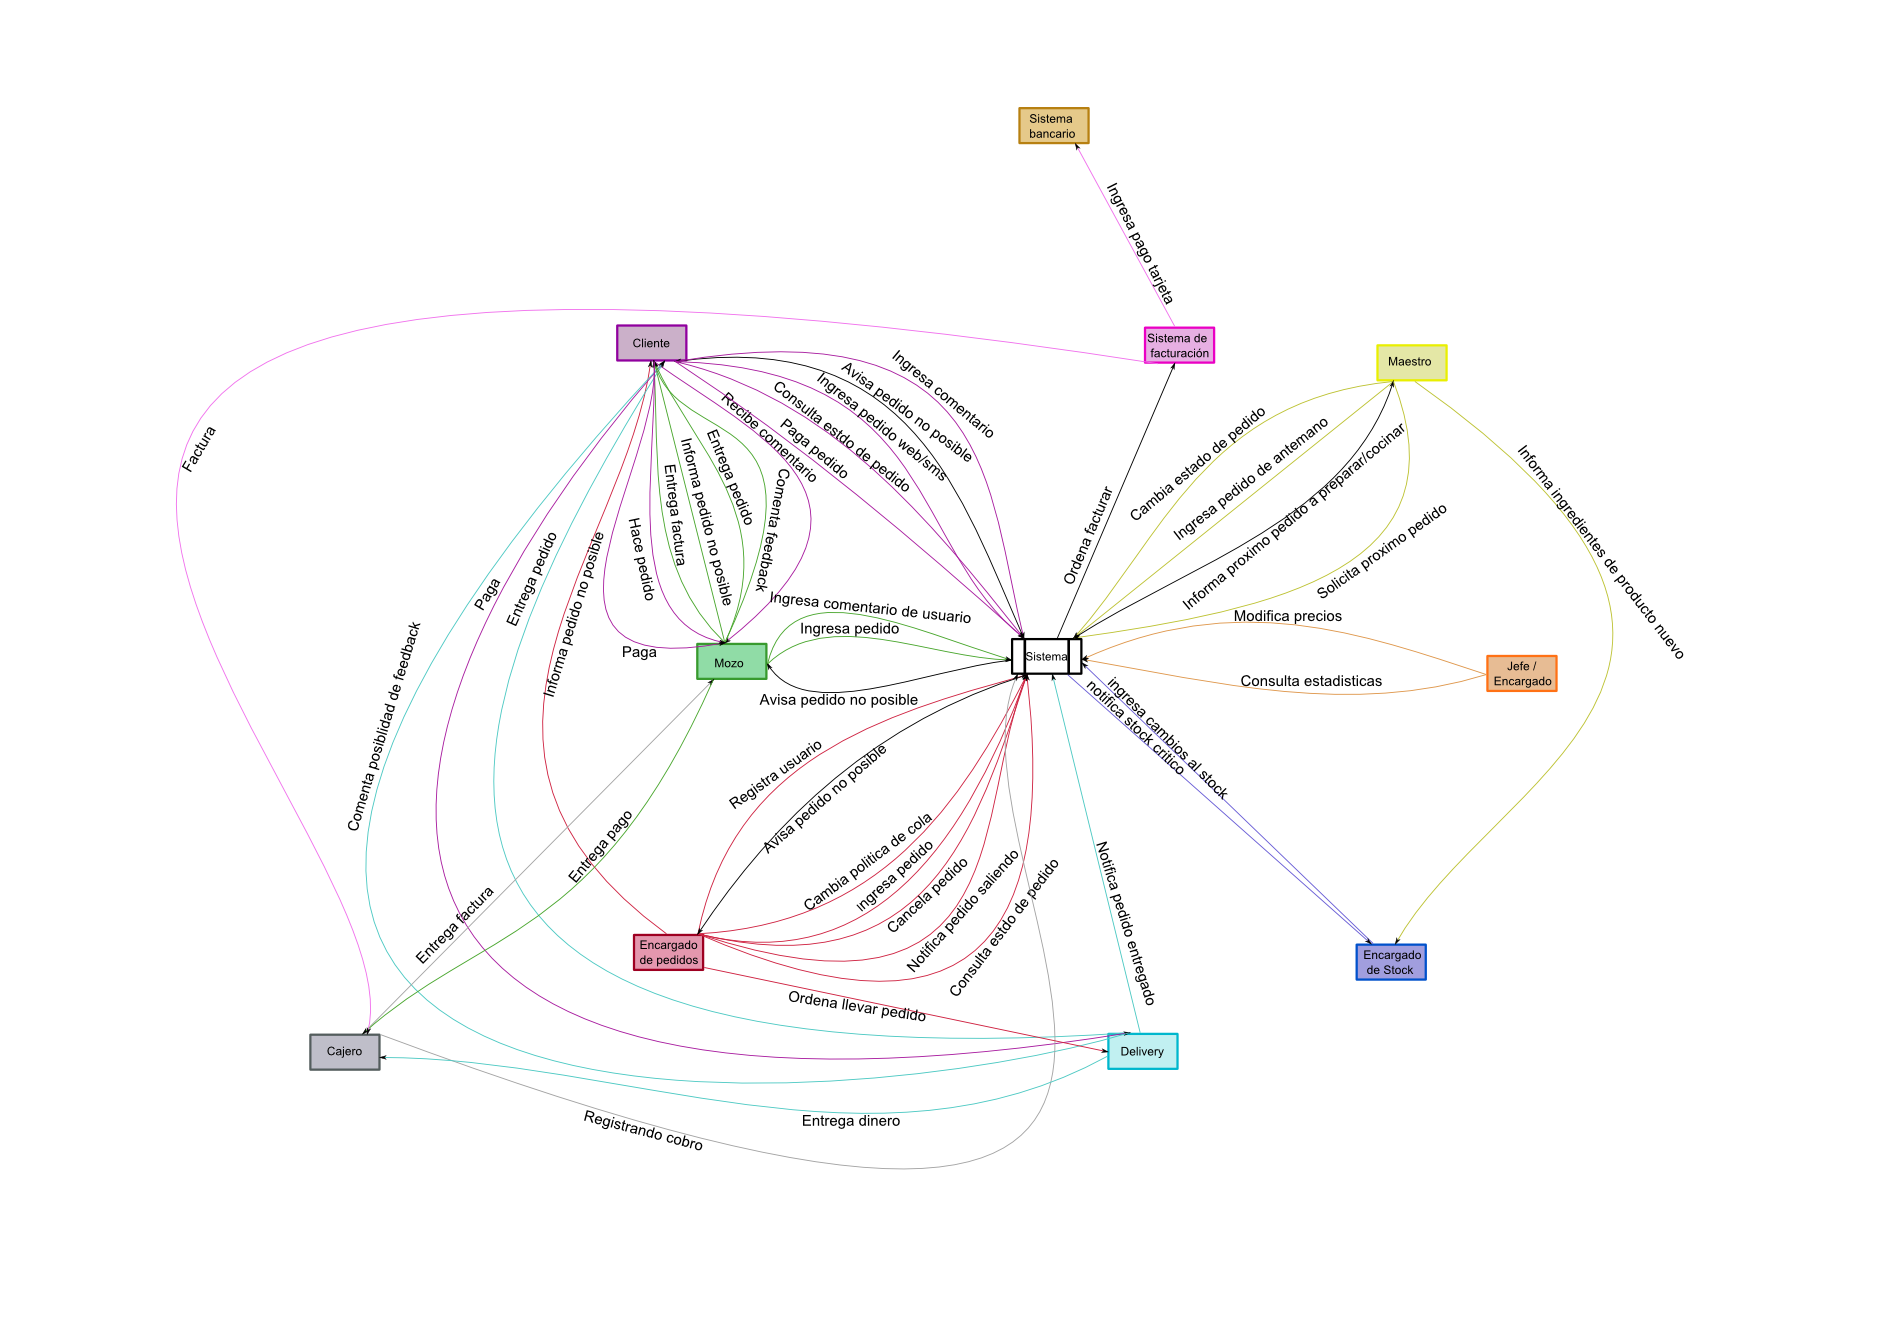
\includegraphics[scale=0.25]{ContextoNormal.png}
\end{figure}
\end{landscape}

\begin{landscape}
\begin{figure}[H]
\centering
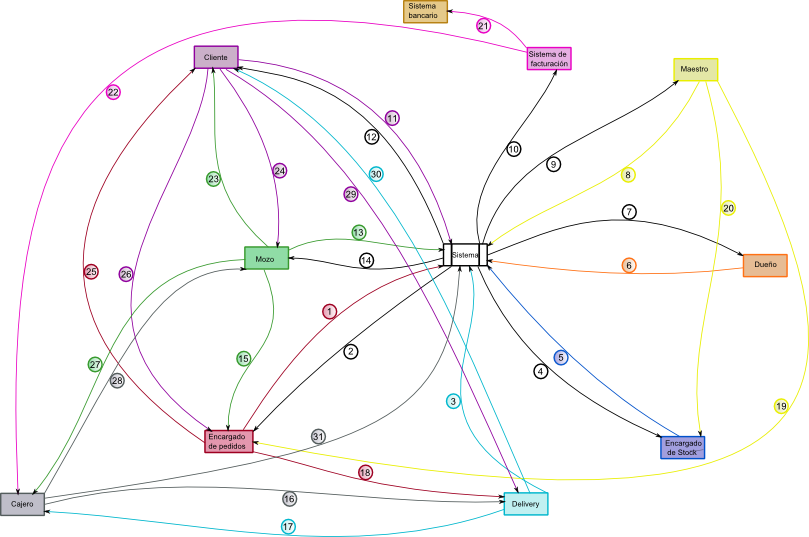
\includegraphics[scale=0.06]{ContextoNormalSimplificado.png}
\end{figure}
\end{landscape}

\begin{minipage}{8cm}
\begin{enumerate}
\item \textcolor{RubineRed}{Encargado de pedidos $\rightarrow$ Sistema}
\begin{itemize}
\item Registra usuarios
\item Ingresa pedidos (diferidos y comunes)
\item Cambia politica de colas
\item Cancela pedidos
\item Notifica pedidos saliendo
\item Consulta estado de pedidos
\end{itemize}
\item \textbf{\textcolor{Black}{Sistema $\rightarrow$ Encargado de pedidos}}
\begin{itemize}
\item Avisa pedido no posible
\item Informa estado de pedidos
\end{itemize}
\item \textcolor{ProcessBlue}{Delivery $\rightarrow$ Sistema}
\begin{itemize}
\item Notifica pedido entregado
\end{itemize}
\item \textbf{\textcolor{Black}Sistema $\rightarrow$ Encargado de stock}
\begin{itemize}
\item Notifica stock critico
\end{itemize}
\item \textcolor{Blue}{Encargado de stock $\rightarrow$ Sistema}
\begin{itemize}
\item Ingresa cambios al stock
\end{itemize}
\item \textcolor{Peach}{Due�o $\rightarrow$ Sistema}
\begin{itemize}
\item Modifica precios
\item Consulta estadisticas
\end{itemize}
\item \textbf{\textcolor{Black}{Sistema $\rightarrow$ Due�o}}
\begin{itemize}
\item Informa estadisticas
\end{itemize}
\item \textcolor{Goldenrod}{Maestro $\rightarrow$ Sistema}
\begin{itemize}
\item Cambia estado de pedidos
\item Solicita proximo pedido
\end{itemize}
\item \textbf{\textcolor{Black}Sistema $\rightarrow$ Maestro}
\begin{itemize}
\item Informa proximo pedido a preparar/cocinar
\end{itemize}
\item \textbf{\textcolor{Black}Sistema $\rightarrow$ Sistema de facturacion}
\begin{itemize}
\item Ordena facturar
\end{itemize}
\item \textcolor{Purple}{Cliente $\rightarrow$ Sistema}
\begin{itemize}
\item Ingresa comentarios
\item Ingresa pedidos via web/sms
\item Consulta estado de pedidos
\item Paga pedido
\end{itemize}
\item \textbf{\textcolor{Black}Sistema $\rightarrow$ Cliente}
\begin{itemize}
\item Avisa pedido no posible
\end{itemize}
\item \textcolor{ForestGreen}{Mozo $\rightarrow$ Sistema}
\begin{itemize}
\item Ingresa pedidos
\end{itemize}
\item \textbf{\textcolor{Black}Sistema $\rightarrow$ Mozo}
\begin{itemize}
\item Avisa pedido no posible
\end{itemize}
\end{enumerate}
\end{minipage}
\ \
\hfill \begin{minipage}{8cm}
\begin{enumerate}
\setcounter{enumi}{14}
\item \textcolor{ForestGreen}{Mozo $\rightarrow$ Encargado de pedidos}
\begin{itemize}
\item Indica cancelacion de pedidos
\end{itemize}
\item \textcolor{Gray}{Cajero $\rightarrow$ Delivery}
\begin{itemize}
\item Entrega Dinero
\end{itemize}
\item \textcolor{ProcessBlue}{Delivery $\rightarrow$ Cajero}
\begin{itemize}
\item Entrega Dinero
\end{itemize}
\item \textcolor{RubineRed}{Encargado de pedidos $\rightarrow$ Delivery}
\begin{itemize}
\item Ordena llevar pedido
\end{itemize}
\item \textcolor{Goldenrod}{Maestro $\rightarrow$ Encargado de pedidos}
\begin{itemize}
\item Ingresa productos preparados de antemano
\end{itemize}
\item \textcolor{Goldenrod}{Maestro $\rightarrow$ Encargado de Stock}
\begin{itemize}
\item Informa ingredientes de producto nuevo
\end{itemize}
\item \textcolor{Rhodamine}{Sistema de facturaci�n $\rightarrow$ Sistema bancario}
\begin{itemize}
\item Ingresa pago tarjeta
\end{itemize}
\item \textcolor{Rhodamine}{Sistema de facturaci�n $\rightarrow$ Cajero}
\begin{itemize}
\item Factura
\end{itemize}
\item \textcolor{ForestGreen}{Mozo $\rightarrow$ Cliente}
\begin{itemize}
\item Entrega pedido
\item Informa pedido no posible
\item Entrega factura
\end{itemize}
\item \textcolor{Purple}{Cliente $\rightarrow$ Mozo}
\begin{itemize}
\item Cancela pedido
\item Hace pedido
\item Paga
\end{itemize}
\item \textcolor{RubineRed}{Encargado de pedidos $\rightarrow$ Cliente}
\begin{itemize}
\item Informa pedido no posible
\end{itemize}
\item \textcolor{Purple}{Cliente $\rightarrow$ Encargado de pedidos}
\begin{itemize}
\item Realiza pedido
\item Cancela pedido
\item Requiere registro
\end{itemize}
\item \textcolor{ForestGreen}{Mozo $\rightarrow$ Cajero}
\begin{itemize}
\item Entrega pago
\end{itemize}
\item \textcolor{Gray}{Cajero $\rightarrow$ Mozo}
\begin{itemize}
\item Entrega factura
\end{itemize}
\item \textcolor{Purple}{Cliente $\rightarrow$ Delivery}
\begin{itemize}
\item Paga
\end{itemize}
\item \textcolor{ProcessBlue}{Delivery $\rightarrow$ Cliente}
\begin{itemize}
\item Entrega pedido
\end{itemize}
\item \textcolor{Gray}{Cajero $\rightarrow$ Sistema}
\begin{itemize}
\item Registra cobro
\item Modifica precios
\item Solicita factura
\end{itemize}
\end{enumerate}
\end{minipage}

\begin{landscape}
\begin{figure}[H]
\centering
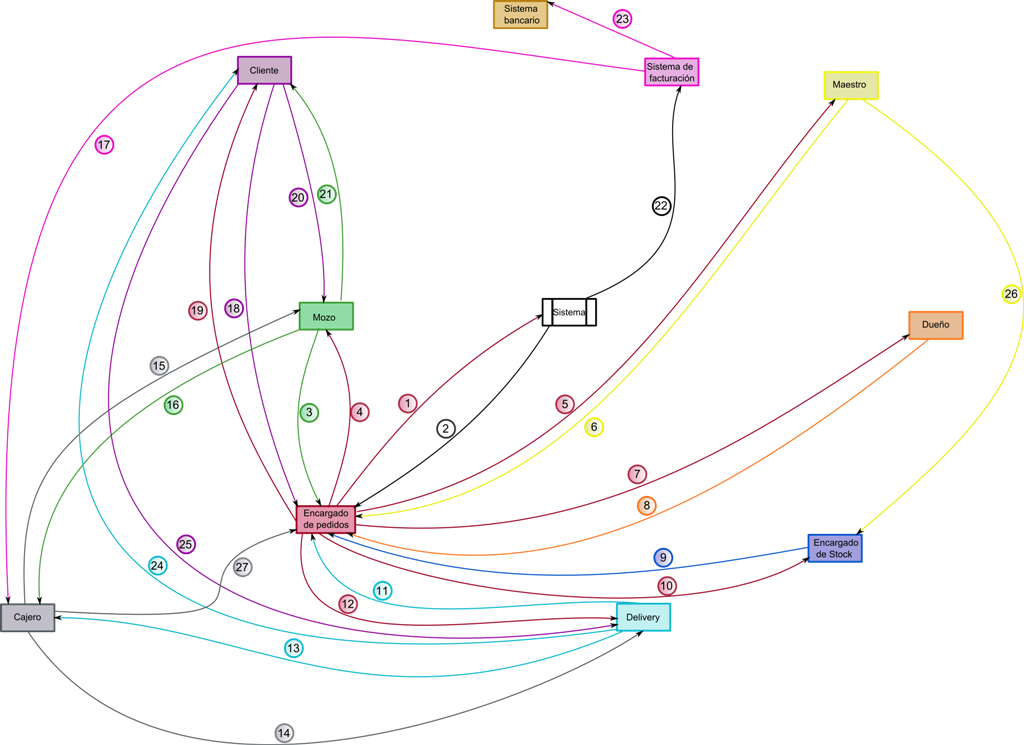
\includegraphics[scale=0.24]{ContextoContingencia.png}
\end{figure}
\end{landscape}

\begin{minipage}{8cm}
\begin{enumerate}
\item \textcolor{RubineRed}{Encargado de pedidos $\rightarrow$ Sistema}
\begin{itemize}
\item Registra usuarios
\item Ingresa pedidos (diferidos y comunes)
\item Cambia politica de colas
\item Notifica pedido saliendo
\item Consulta estado de pedido
\item Cambia estado de pedido
\item Modifica precios
\item Consulta estadisticas
\item Ingresa cambios al stock
\item Registra Cobro
\item Solicita factura
\end{itemize}
\item \textbf{\textcolor{Black}{Sistema $\rightarrow$ Encargado de pedidos}}
\begin{itemize}
\item Avisa pedido no posible
\item Informa estado pedidos
\item Informa estadisticas
\item Notifica stock critico
\item Informa prox pedido a preparar/cocinar
\end{itemize}
\item \textcolor{ForestGreen}{Mozo $\rightarrow$ Encargado de pedidos}
\begin{itemize}
\item Notifica pedidos hechos
\item Indica cancelacion
\end{itemize}
\item \textcolor{RubineRed}{Encargado de pedidos $\rightarrow$ Mozo}
\begin{itemize}
\item Avisa pedido listo para entregar
\item Avisa pedido no posible
\end{itemize}
\item \textcolor{RubineRed}{Encargado de pedidos $\rightarrow$ Maestro}
\begin{itemize}
\item Ordena proximo pedido a preparar/cocinar
\end{itemize}
\item \textcolor{Goldenrod}{Maestro $\rightarrow$ Encargado de pedidos}
\begin{itemize}
\item Notifica estado de pedidos
\item Entrega pedido preparado
\item Ingresa productos preparados de antemano
\end{itemize}
\item \textcolor{RubineRed}{Encargado de pedidos $\rightarrow$ Due�o}
\begin{itemize}
\item Informa estadisticas
\end{itemize}
\item \textcolor{Peach}{Due�o $\rightarrow$ Encargado de pedidos}
\begin{itemize}
\item Ordena modificar precios
\item Pide informe de estadisticas
\end{itemize}
\item \textcolor{Blue}{Encargado de stock $\rightarrow$ Encargado de pedidos}
\begin{itemize}
\item Informa cambios de stock
\end{itemize}
\item \textcolor{RubineRed}{Encargado de pedidos $\rightarrow$ Encargado de stock}
\begin{itemize}
\item Informa stock critico
\end{itemize}
\item \textcolor{ProcessBlue}{Delivery $\rightarrow$ Encargado de pedidos}
\begin{itemize}
\item Notifica pedido entregado y pagado
\end{itemize}
\item \textcolor{RubineRed}{Encargado de pedidos $\rightarrow$ Delivery}
\begin{itemize}
\item Ordena llevar pedido
\end{itemize}
\end{enumerate}
\end{minipage}
\ \
\hfill \begin{minipage}{8cm}
\begin{enumerate}
\setcounter{enumi}{12}
\item \textcolor{ProcessBlue}{Delivery $\rightarrow$ Cajero}
\begin{itemize}
\item Entrega dinero
\end{itemize}
\item \textcolor{Gray}{Cajero $\rightarrow$ Delivery}
\begin{itemize}
\item Da la factura para la entrega
\end{itemize}
\item \textcolor{Gray}{Cajero $\rightarrow$ Mozo}
\begin{itemize}
\item Entrega factura
\end{itemize}
\item \textcolor{ForestGreen}{Mozo $\rightarrow$ Cajero}
\begin{itemize}
\item Entrega pago
\end{itemize}
\item \textcolor{Rhodamine}{Sistema de facturaci�n $\rightarrow$ Cajero}
\begin{itemize}
\item Factura
\end{itemize}
\item \textcolor{Purple}{Cliente $\rightarrow$ Encargado de pedidos}
\begin{itemize}
\item Realiza pedido por telefono
\item Cancela pedido por telefono
\item Requiere registro
\item Consulta estado de pedido
\end{itemize}
\item \textcolor{RubineRed}{Encargado de pedidos $\rightarrow$ Cliente}
\begin{itemize}
\item Informa pedido no posible
\item Informa estado de pedido
\end{itemize}
\item \textcolor{Purple}{Cliente $\rightarrow$ Mozo}
\begin{itemize}
\item Hace pedido
\item Paga
\item Cancela pedido
\end{itemize}
\item \textcolor{ForestGreen}{Mozo $\rightarrow$ Cliente}
\begin{itemize}
\item Informa pedido no posible
\item Entrega factura
\item Entrega pedido
\end{itemize}
\item \textbf{Sistema $\rightarrow$ Sistema de facturaci�n}
\begin{itemize}
\item Ordena facturar
\end{itemize}
\item \textcolor{Rhodamine}{Sistema de facturaci�n $\rightarrow$ Sistema bancario}
\begin{itemize}
\item Ingresa pago tarjeta
\end{itemize}
\item \textcolor{ProcessBlue}{Delivery $\rightarrow$ Cajero}
\begin{itemize}
\item Entrega pedido
\end{itemize}
\item \textcolor{Purple}{Cliente $\rightarrow$ Mozo}
\begin{itemize}
\item Paga
\end{itemize}
\item \textcolor{Goldenrod}{Maestro $\rightarrow$ Encargado de pedidos}
\begin{itemize}
\item Informa ingredientes de nuevo producto
\item Entrega pedido preparado
\item Ingresa productos preparados de antemano
\end{itemize}
\item \textcolor{Gray}{Cajero $\rightarrow$ Encargado de pedidos}
\begin{itemize}
\item Avisa registrar cobro
\item Avisa solicita factura
\item Modifica precios
\end{itemize}
\end{enumerate}
\end{minipage}
\chapter{Casos de uso}
\section{Diagrama}
\newpage
\begin{figure}[H]
\centering
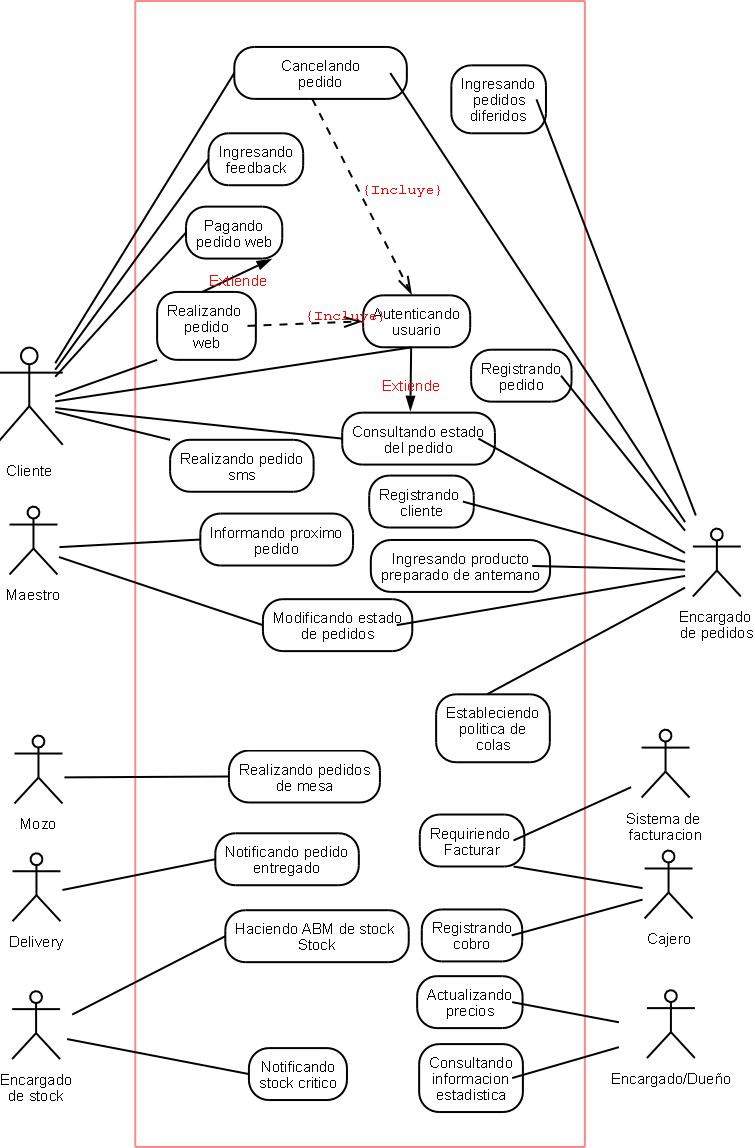
\includegraphics[scale=0.4]{casosdeuso.png}
\end{figure}

\section{Breve descripci�n}
A continuaci�n daremos a modo ilustrativo una breve descripci�n de los casos de uso 
considerados en el diagrama. La misma no pretende ser exahustiva, sino simplemente presentar 
un panorama de a qu� se refiere cada caso de uso.

\setcounter{subsection}{0}
\subsection{Autenticando usuario}

\textit{Agente: Cliente}

Para poder acceder a los distintos servicios v�a Web que ofrece la pizzer�a, es necesario 
que el usuario se identifique. Para obtener una cuenta de usuario, el mismo tendr� que 
registrarse personal o telef�nicamente.

Este caso de uso est� relacionado con el objetivo de lograr ampliar la forma de registro de 
pedidos, as� como tambi�n ayuda a poder lograr que los usuarios consulten 
el estado de los mismos y lo paguen v�a Internet.

\subsection{Realizando pedido v�a Web}

\textit{Agente: Cliente}

El usuario, una vez autenticado, puede armar un pedido a trav�s de la p�gina Web de la 
pizzer�a. Una vez elegidos los productos que desea ordenar, podr� optar por pagarlo en 
efectivo al \textit{delivery} o pagar por Internet con su tarjeta de cr�dito. Adem�s, el sistema le dar� alg�n 
identificador de pedido que le permita consultar el estado del mismo. Si el pedido no se 
puede armar porque no hay productos para hacerlo, el sistema mostrar� un mensaje al usuario.

Este caso de uso sirve para poder lograr ampliar la forma de hacer pedidos por parte de los 
clientes.

\subsection{Pagando v�a web}

\textit{Agente: Cliente}

El usuario al realizar un pedido puede elegir hacer un pago v�a Web utilizando su tarjeta 
de cr�dito.

Este caso de uso es tambi�n necesario para poder lograr que los usuarios hagan pedidos de 
varias formas.

\subsection{Cancelando pedido}

\textit{Agente: Encargado de pedidos}

Este caso de uso permite que en cualquier momento el encargado pueda cancelar un pedido
que fue ingresado previamente al sistema, sin importar su estado. La cancelaci�n puede
tener motivos varios, aunque lo m�s com�n sea hacerlo a pedido del cliente.

Este caso de uso es �til para permitir que los usuarios tengan una interaccion m�s fluida 
con la pizzer�a, as� como facilitar la integraci�n del sistema con el modelo de producci�n.

\subsection{Realizando pedido v�a SMS}

\textit{Agente: Cliente}

Como alternativa al pedido telef�nico, Web o personal, es posible hacer un pedido mediante 
SMS. Para esto el usuario tiene que haberse registrado anteriormente. Para hacerlo, se 
utilizan c�digos que permiten identificar qu� quiere el usuario. Si no se puede hacer el 
pedido, se enviar� un mensaje al usuario notific�ndolo de la situaci�n.

Este caso de uso ayuda a lograr nuevas formas de registrar pedidos por parte de los usuarios.

\subsection{Ingresando feedback}

\textit{Agente: Cliente}

Una vez realizada la entrega de un pedido por \textit{delivery}, el usuario tiene la posibilidad de 
opinar sobre el servicio mediante Internet. Para esto no es necesario que el usuario se
loguee ya que utiliza para ello un c�digo �nico que recibe al momento de entrega del
pedido.

Esta informaci�n u opiniones sobre el servicio ayudan a lograr informaci�n estad�stica sobre 
el funcionamiento de la pizzer�a, que podr�a usarse para identificar posibles conflictos 
en la misma o para generar promociones.

\subsection{Consultando estado de pedido}

\textit{Agentes: Cliente, encargado de pedidos}

El cliente, v�a web, o el encargado de pedidos en su computadora, pueden consultar el estado 
de un pedido. El cliente tiene que loguearse previamente.

Este caso de uso ayuda a lograr que los usuarios puedan conocer el estado de su pedido, as�
como tambi�n a conocer informaci�n de seguimiento y control de los pedidos.

\subsection{Ingresando pedidos diferidos}

\textit{Agente: Encargado de pedidos}

Luego de una ca�da del sistema, cuando �ste vuelve a levantarse, el encargado de pedidos 
puede ingresar los pedidos que se tomaron mientras el sistema no estuvo disponible. Este 
caso de uso es diferente del ingreso de pedidos normales, porque un pedido 
diferido puede ya haber sido entregado al momento de registrarse, de modo que esto debe poder 
diferenciarse.

El ingreso de pedidos diferidos permite mantener la informaci�n sobre los pedidos, a fin de 
poder lograr informaci�n estad�stica precisa.

\subsection{Ingresando producto preparado de antemano}
\textit{Agente: Encargado de pedidos}

El maestro de cocina podr�a en momentos donde el trabajo de la pizzer�a es bajo, preparar 
alg�n producto para luego en caso de un futuro pedido no ya tenerlo preparado.

Este caso de uso ayuda a lograr mejor atenci�n a los clientes, y es una propuesta nuestra 
para mejorar la operatoria actual.

\subsection{Estableciendo pol�tica de colas}
\textit{Agente: Encargado de pedidos}

El encargado de pedidos puede modificar la pol�tica de cola de pedidos, as� como tambi�n 
modificar el orden en el que ser�n preparados los pedidos.

Este caso de uso ayuda a satisfacer el objetivo de controlar la pol�tica de cola de pedidos.

\subsection{Registrando pedido}

\textit{Agente: Encargado de pedidos}

El encargado de pedidos ingresa un nuevo pedido de un llamado telef�nico. El software le 
informa la planificaci�n existente y los tiempos estimados de cocci�n. 
%esta en el enunciado aunque queda de los pelos no lo nombramos en ningun otra parte.

Este caso de uso est� relacionado con lograr automatizar la operatoria. Adem�s, al ingresar 
los pedidos se hace posible lograr informaci�n estad�stica.

\subsection{Registrando cliente}
\textit{Agente: Encargado de pedidos}

El encargado de pedidos ingresa un nuevo cliente al sistema, el cual se comunica con el 
encargado v�a tel�fono o personalmente. Para hacerlo, toma los datos del mismo.

Este caso de uso permite que posteriormente se realicen pedidos v�a Web o v�a SMS.

\subsection{Informando pr�ximo pedido}

\textit{Agente: Maestro}

El maestro pide al sistema el pr�ximo pedido a preparar, as� como tambi�n el proximo pedido 
a ingresar al horno.

Este caso de uso ayuda a automatizar la operatoria de la pizzer�a y automatizar la asignaci�n 
de horno.

\subsection{Modificando estado de pedido} 
%TODO: verificar cuando el maestro actualiza el estado del pedido
\textit{Agentes: Maestro, Encargado de pedidos}

Este caso de uso permite actualizar en qu� etapa del ciclo de pedidos se encuentra un 
pedido. El maestro actualiza el estado del pedido cuando lo comienza a preparar, cuando 
termina de prepararlo, al ingresarlo al horno y cuando est� listo. El encargado de pedidos actualiza el 
estado cuando el pedido se despacha para su entrega.

Este caso de uso permite tener informaci�n de seguimiento y control de los pedidos 

\subsection{Ingresando pedido de mesa}

\textit{Agente: Mozo}

El mozo cuenta con una PDA a fin de ingresar los pedidos que le hacen en las mesas al 
sistema.

Este caso de uso permite ampliar el acceso al software, automatizar la operatoria y lograr 
un mejor servicio a los clientes, y es un agregado que proponemos para mejorar la operatoria 
de la pizzer�a.

\subsection{Notificando pedido entregado}

\textit{Agente: Delivery}

El \textit{delivery} deber� informar mediante SMS cuando realiza una entrega, de modo que el sistema 
actualice el estado del pedido a entregado.

Este caso de uso es tambi�n un agregado que proponemos para mejorar la operatoria de la
pizzer�a, y permite lograr informaci�n estad�stica (por ejemplo demora de la entrega) as�
como tambi�n informacion de seguimiento y control de los pedidos.

\subsection{Haciendo ABM de stock}

\textit{Agente: Encargado de stock}

El responsable de controlar el stock de las materias primas y kits en la pizzer�a tendra la capacidad
de actualizar el stock ya sea dando de alta productos comprados as� como tambi�n dando de baja
productos caducados. Por otro lado, podr� en cualquier momento consultar el stock de los productos y kits.

El caso de uso ayuda a lograr controlar el stock de la pizzer�a.

\subsection{Notificando stock cr�tico}

\textit{Agente: Encargado de stock}

En caso de que el stock de algun producto quede por debajo de un nivel cr�tico, 
el sistema avisar� al encargado de stock de esta situaci�n.

Esta funcionalidad permite controlar el stock, y adem�s satisface el pedido expl�cito de 
que el sistema avise en caso de stock inferior al nivel cr�tico.

\subsection{Actualizando precios}

\textit{Agente: Cajero, due�o}

Tanto el due�o como el encargado de caja pueden modificar los precios de los distintos productos 
en cualquier momento. 
%fixme: cuando se ven dichos cambios.

El caso de uso satisface el requerimiento expl�cito de poder modificar precios y permite 
adem�s poder lograr promociones y precios competitivos.

\subsection{Consultando informaci�n estadistica}

\textit{Agente: Due�o}

El due�o puede consultar la informaci�n estadistica sobre los 
pedidos y el funcionamiento de la pizzer�a.

El caso de uso satisface el requerimiento expl�cito de poder consultar informacion estad�stica 
a fin de lograr precios competitivos y promociones.

\subsection{Registrando cobro}

\textit{Agente: Cajero}

Cuando se cobra un pedido o el \textit{delivery} entrega el dinero, se registra el pago del pedido. 
Este registro es ingresado manualmente por el cajero.

Esta funcionalidad permite manterner informaci�n sobre el estado de los pedidos.

\subsection{Requiriendo facturar}

\textit{Agentes: Cajero, sistema de facturaci�n}

El cajero debe requerir que se emita factura cuando se paga un pedido o cuando este sale 
para ser entregado por el \textit{delivery}. El sistema interact�a con el software de 
facturaci�n por medio de la interfaz que este presenta para lograr la facturaci�n.

Este caso de uso permite interactuar con el sistema de facturaci�n sin tener que 
ingresar nuevamente los datos del pedido.


\chapter{Glosario}
\section{Terminolog�a}
\begin{itemize}
\item \textbf{Pedido:} Se denomina ``pedido'' a todo pedido realizado por un cliente 
(a trav�s de alguno de los medios de contacto disponibles) y que ya ha sido 
procesado por el sistema. Un pedido no es tal, y no se registra informaci�n sobre �l,
hasta el momento en que se da de alta en el sistema.
\item \textbf{Encargado de pedidos:} El encargado de pedidos es un empleado cuya labor es la de administrar los pedidos y el funcionamiento generascontrola la facturaci�n y supervisa la distribuci�n de los pedidos. Adem�s tiene privilegios para situaciones especiales (reorganizaci�n de la cola de pedidos, cambios de pol�tica de pedidos, cancelaciones y acceso al ABM de usuarios). En caso de contingencia (sistema ca�do o con funcionalidad limitada), este agente deber� controlar el funcionamiento manual del sistema y posteriormente ingresar los datos de los pedidos recibidos para su registro en el sistema.
\item \textbf{Encargado de stock:} El encargado de stock es la persona responsable de
recibir las notificaciones relacionadas a los niveles de stock e ingresar los datos
respectivos a las altas y bajas del stock. En la mec�nica actual de la pizzer�a no
hay un encargado de stock definido. Si bien su papel ser� desempe�ado por alguno
de los otros agentes (due�o o encargado de pedidos), decidimos separar su rol puesto 
que se trata de una tarea independiente de las dem�s.
\item \textbf{Cajero:} El cajero se encarga de modificar los precios (capacidad que
comparte con el due�o), registrar los pagos que se hacen en el local, recibir el dinero
del \textit{delivery} e ingresar los pagos en el sistema, y solicitar la facturaci�n
de pedidos cuando sea necesario.
\item \textbf{Due�o:} El due�o es responsable de la gesti�n de la carta de la pizzer�a, sus precios y es el interesado en acceder a las estad�sticas sobre el funcionamiento del negocio.
\item \textbf{Cocinero:} El cocinero es cualquier persona que trabaja en la cocina. En principio es ya sea el maestro pizzero o el maestro empanadero, pero podr�a ser un ayudante de cocina en general.
\item \textbf{Estad�sticas:} Las estad�sticas son registros hist�ricos de los indicadores de rendimiento, que permiten evaluar la progresi�n del negocio a lo largo del tiempo.
\item \textbf{Indicadores de rendimiento:} Son valores num�ricos que describen el rendimiento de la pizzer�a en un per�odo determinado. Pueden depender de factores diversos. Algunos ejemplos de indicadores de rendimiento son la tasa de producci�n de la cocina, la tasa de ocupaci�n del horno, el tiempo medio de espera por un pedido o la cantidad de valoraciones negativas obtenidas por el sistema de feedback. Algunos de ellos se le presentan al encargado de pedidos en tiempo real.
\item \textbf{Maestro Pizzero:} Es el cocinero encargado de las pizzas, que se ocupa de determinar los ingredientes que componen a una pizza dada, prepararla y supervisar su cocci�n si se hace en su horno. En el contexto del sistema, es responsable de los cambios de estado de los pedidos en la secci�n que concierne a la cocina.
\item \textbf{Maestro Empanadero:} An�logo al maestro pizzero pero para la preparaci�n de empanadas.
\item \textbf{Mesero o Mozo:} Es el responsable de atender a los clientes en las mesas y registrar sus pedidos en el PDA que luego los transfiere al sistema. Si el sistema est� degradado y no dispone del PDA, registrar los pedidos mentalmente o en papel y luego se los entrega al encargado de pedidos.
\item \textbf{Cliente:} Es cualquier individuo que est� interesado en adquirir productos de la pizzer�a, a trav�s de cualquiera de los medios de contacto y pedido.
\item \textbf{Cliente local:} Cliente que concurre personalmente al local y es atendido por un mesero en su mesas.
\item \textbf{Cliente remoto:} Cliente que hace su pedido desde su casa u otro lugar y requiere que le sea entregado por el servicio de delivery.
\item \textbf{Cliente telef�nico:} Cliente remoto que realiza su pedido por tel�fono (es atendido por el encargado de pedidos que a su vez ingresa el pedido en el sistema manualmente.
\item \textbf{Cliente Web:} Cliente remoto que realiza su pedido a trav�s de la p�gina web de la pizzer�a. El sistema registra su pedido sin ninguna intervenci�n humana.
\item \textbf{Cliente SMS:} Cliente remoto que realiza su pedido a trav�s de mensajes de texto. El sistema registra su pedido sin ninguna intervenci�n humana.
\item \textbf{Servicio de delivery:} Servicio de entrega a domicilio de los pedidos. Este servicio se subcontrata a un tercero que provee toda la log�stica de entregas, debiendo la pizzer�a �nicamente indicar las entregas que deben realizarse.
\item \textbf{Cola de pedidos:} La cola de pedidos almacena los pedidos que deben prepararse y entregarse, y permite priorizarlos seg�n la pol�tica de cola elegida. Dichar priorizaci�n puede ser manual o autom�tica. 
\item \textbf{Pol�tica de cola:} La pol�tica de cola es el criterio que se utiliza para determinar la ubicaci�n de los pedidos en la cola de pedidos. En general se utiliza este t�rmino para denominar a un criterio algor�timico automatizado de ordenamiento de los pedidos, pero la pol�tica puede ser algo tan simple como ``el encargado de pedidos ordena la cola de pedidos''.
\item \textbf{Sistema de facturaci�n:} Es un sistema inform�tico externo que mediante una interfaz predefinida se encarga de la facturaci�n y emisi�n de comprobantes de todas las ventas que se producen en la pizzer�a.
\item \textbf{Sistema de SMS:} Es un sistema inform�tico externo que provee un servicio de interfaz con las empresas de telefon�a celular, permitiendo que el sistema procese mensajes que los clientes env�an a trav�s de SMS.
\item \textbf{Pedido diferido:} Los pedidos diferidos son pedidos que se realizaron por fuera del sistema (por diversas razones, una de las cuales puede ser una ca�da del sistema). Se permite al encargado registrar dichos pedidos despu�s de que fueron procesados manualmente para que sean tenidos en cuenta en las estad�sticas.
\item \textbf{Productos preparados de antemano:} En alguna situaciones pueden prepararse los productos de antemano dej�ndolos listos para ingresar al horno, antes de que los pedidos sean efectuados. Esto permite preparar la cocina para un pico de demanda. Es importante no confundir con las materias primas necesarias para la preparaci�n.
\end{itemize}

\section{Estados de pedido}
Los estados en los que puede encontrarse un pedido una vez que ingres� al sistema son:
\begin{itemize}
\item Ingresado: El pedido pas� los chequeos necesarios, se determin� que es posible llevarlo a cabo con �xito y se ingres� al sistema, yendo a parar a una cola donde espera a que la cocina est� lista para prepararlo.
\item	En preparaci�n: El pedido ya fue recibido por la cocina y est� siendo preparado por un cocinero.
\item	Preparado: El pedido ya fue preparado en su totalidad y est� listo para ingresar al horno cuando haya lugar disponible.
\item	En el horno: El pedido (o al menos una de sus partes) est� en el horno.
\item	Listo: El pedido est� listo para ser entregado al cliente.
\item	Enviado: El pedido fue entregado al delivery para su entrega a domicilio.
\item	Finalizado: El pedido fue entregado con �xito (ya sea a la mesa o a domicilio).
\item	Cancelado: El pedido fue cancelado antes de su entrega.
\end{itemize}
\begin{figure}
\centering
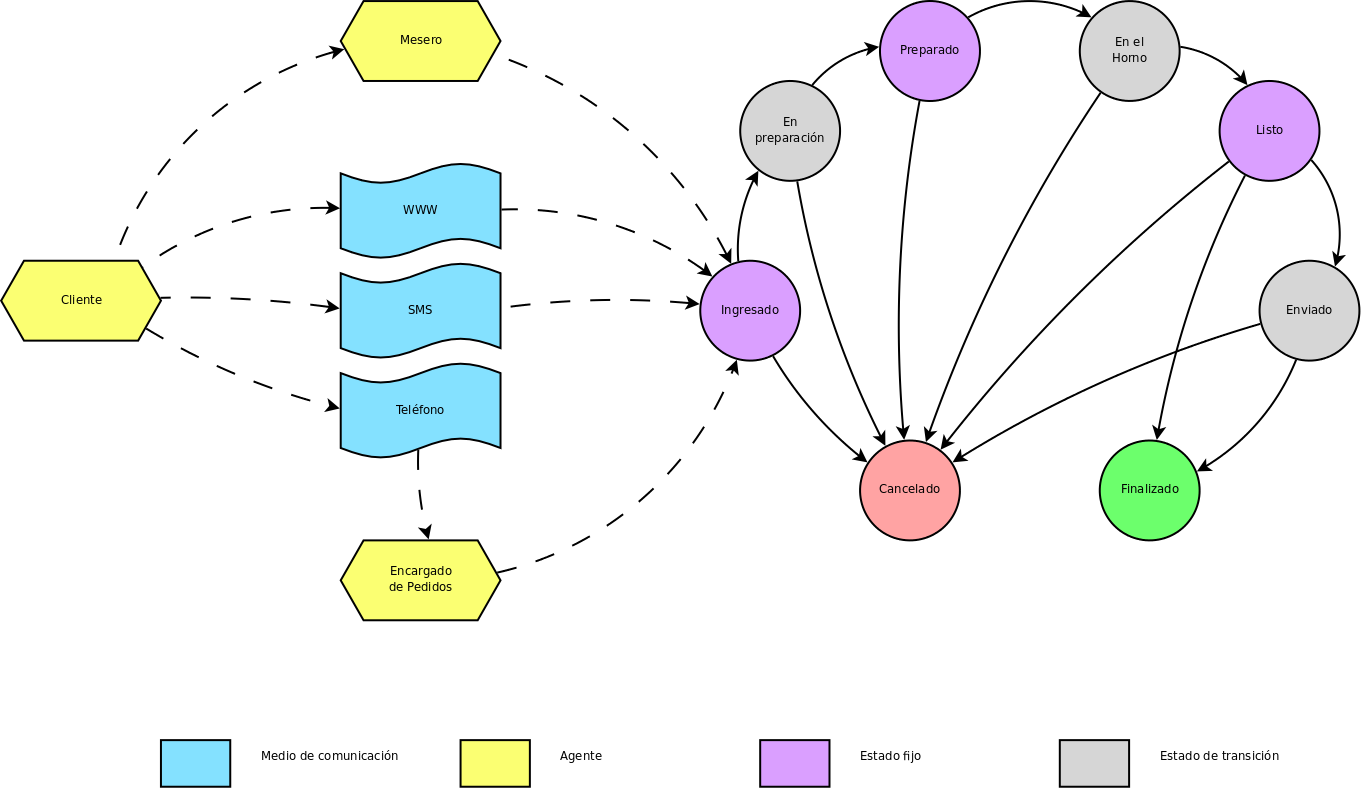
\includegraphics[scale=0.25]{ciclo_pedido.png}
\end{figure}

En breve, un proceso ingresa al sistema cuando es requerido por un cliente por alg�n medio de comunicaci�n. Enseguida se indica a la cocina que el pedido debe ser preparado. Una vez completada la preparaci�n de la comida, los responsables de cocina lo indican al sistema que planifica de forma independiente la asignaci�n de lugares en los hornos. Finalmente, despu�s de que el pedido es horneado, se entrega a la mesa o al delivery seg�n corresponda. Por �ltimo cuando existe confirmaci�n de la entrega se marca el pedido como finalizado y se almacena con fines de registro. El pedido puede ser cancelado en cualquier punto (salvo despu�s de ser finalizado), con implicaciones varias en el sistema de control de stock.

Los estados presentados tienen utilidad para el sistema puesto que hay necesidad de indicar al cliente sobre el estado de su pedido. As�, se podr� indicar si un pedido est� siendo preparado o ya fue enviado al destinatario. Si bien para estos fines alcanza con 3 estados (preparando, enviando, finalizado), se agregan los dem�s con fines de control para el sistema. Adem�s, la granularidad m�s fina permite al sistema hacer predicciones y organizaciones m�s eficientes del uso de los recursos. Por ejemplo, al controlar los tiempos de preparaci�n por separado de los de horneado resulta m�s sencillo, en caso de un cuello de botella en la cocina, determinar cual es el factor limitante.

\label{LastPage}
\end{document}